
%-------------------------------------------------------------------------%
\section{The Standard Model}
The Standard Model (SM) consists of three generations of matter as \textit{fermions} of spin-$1/2$ and three fundamental forces\footnote{Electromagnetism, the Weak force and the Strong force. gravity is not yet fully understood at the quantum scale, therefore it is not included in the SM.} including the Higgs as \textit{bosons}\footnote{The Higgs Boson is spin-0, whereas the other bosons are spin-1.}. The three fundamental forces interact with the fermionic matter through its own unique corresponding Quantum Field Theory (QFT), in which the interaction of matter with the Higgs field provides the masses to such particles as we measure to date. \\

Fermionic matter consists of \textit{leptons} and \textit{quarks}, in which Table \ref{tab:SMFerm} depicts. Each of the three generations of quarks have an up-type and a down-type quark categorized by their charges ($+2/3 \text{ or } -1/3$), and the leptons consist of charged and neutral leptons in which the neutral components are known as neutrinos. The up-type quarks are the \textit{up}, \textit{charm} and \textit{top} quarks, and the down-type quarks are the \textit{down}, \textit{strange} and \textit{bottom} quarks. These quarks, except for the top quark, exist in a bound state known as \textit{hadrons} and can never be observed directly. Hadrons are categorized into mesons or (anti-)bayons\footnote{Mesons consist of two quarks; one quark and anti-quark each. (Anti-)Baryons consist of three (anti-)quarks.} in which the proton and neutrons are a family of \cite{thomson2013modern}. The first generation of elementary particles represent the basic building blocks of the low energy Universe, and more complex interactions are mediated by the second and third generations \cite{thomson2013modern}. Furthermore, these particles differ greatly in mass where the later generations are much heavier than the first. \\

\begin{table}[htbp]
    \centering
    \begin{tabular}{||c|c|c|c||}
    \hline
    & Gen1 & Gen2 & Gen3 \\
    \hline
    \multirow{2}{1.2cm}{quarks} & $u$ & $c$ & $t$ \\
     & $d$ & $s$ & $b$ \\
    \hline
    \multirow{2}{1.2cm}{leptons} & $e$ & $\mu$ & $\tau$ \\
     & $\nu_e$ & $\nu_\mu$ & $\nu_\tau$ \\
    \hline
    \end{tabular}
    \caption{The three generation of fermionic matter in the Standard Model. From the top row, left to right, we have the up, charm, top, down, strange and bottom quarks, followed by the electron, muon and tau for the charged leptons and their associated neutrinos as neutral leptons. All fermions in this table have spin-$1/2$.}
    \label{tab:SMFerm}
\end{table}


The gauge bosons consist of four vector bosons in the form of \textit{gluons}, \textit{photons}, \textit{Z bosons} (neutrally-charged) and \textit{W bosons} (electrically charged). The photon mediates electromagnetism (QED) and the gluons mediate the strong force (QCD) where the interactions in theory relies on them being mass-less, which are already experimentally verified. The weak force is mediated by the Z and W bosons, which are massive; roughly 80 and 91GeV/c$^2$ respectively, to be precise \cite{tanabashi2018review}. The weak gauge bosons and the photon are `produced' through the Higgs mechanism and electroweak symmetry breaking. In essence, the Higgs field which is a doublet that contains a neutral and a charged component, acquires some vacuum expectation value (vev) which produces a physical Higgs and some massless Goldstone bosons. This is known as the Higgs mechanism. Through broken symmetries and mixing, the photon arises from the $B$, the $Z^0$ arises from $W^3$ and the $W^\pm$ arises from the $W^1 \pm iW^2$ components of the electroweak Lagrangian's field tensors \cite{thomson2013modern}. These terms will be relevant again when we touch on supersymmetry. \\

\begin{table}[htbp]
    \centering
    \begin{tabular}{||c|c||}
    \hline
       Gauge Bosons  & Scalar Bosons \\
     \hline
       $g$, $\gamma$ ($B$), $Z^0$ ($W^3$), $W^\pm$ & $H^0$ \\
     \hline
    \end{tabular}
    \caption{Force carriers (bosons) in the Standard Model. The gauge bosons consist of the gluon, photon, Z boson and W bosons, where the photon and Z boson originate from the $B$ and the $W^3$ components. The Higgs boson is the only known scalar in the SM with spin-0, opposed to the gauge bosons that are vector bosons and have spin-1.}
    \label{tab:SMBos}
\end{table}


%-------------------------------------------------------------------------%
\section{The top quark and its decay}
Amongst the SM particles, the top quark interests us the most as this will correspond to our background events.  The top quark has a rest mass of $m_t\approx175\text{GeV/c}^2$ and an electric charge of +2/3$e$ \cite{tanabashi2018review} making it the only known elementary particle in the SM to be heavier than the Higgs boson. The theoretical predictions of top quarks and the bottom quark was established in 1973 by Kobayashi and Masakawa to explain charge-parity (CP) violation in some meson decays \cite{griffiths2008introduction, kobayashi1973cp}. Experimental evidence for the bottom quark, the generationally paired particle to the top quark, was found at Fermilab in 1977 \cite{herb1977observation}. Nearly two decades later in 1994, the top quark was discovered at the Tevatron with an energy\footnote{The Centre-of-Mass energy, denoted as $\sqrt{s}$, is a Lorentz invariant value such that $s=\Big( \sum\limits_{i=1}^2 E_i \Big)^2 - \Big( \sum\limits_{i=1}^2 \overrightarrow{p_i} \Big)^2 $. Note that $c=1$ and each $i$ represents the protons in the beam.} of $\sqrt{s}=1.8\text{TeV}$ through the process $p\Bar{p} \rightarrow t\Bar{t}$ \cite{abachi1994search, coll1994evidence, abachi1995observation}. The top quark almost always decays through the weak interaction into a bottom quark and a W boson pair. The W boson then produces a charged lepton-neutrino pair or a pair of quark-antiquark that form hadronic jets. These possible decay modes are given in Figure \ref{fig:topdecay}. \\

\begin{figure}[htbp]
    \centering
    \begin{minipage}{0.24\linewidth}
        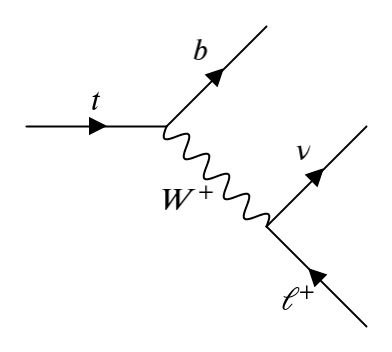
\includegraphics[width=\linewidth]{top1.png}
        \label{fig:top1}
    \end{minipage}
    \begin{minipage}{0.24\linewidth}
        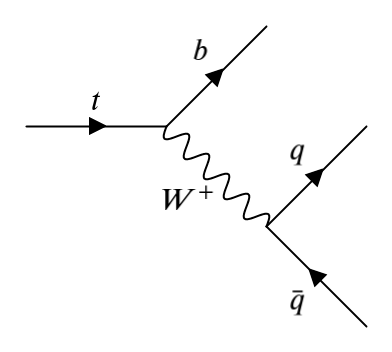
\includegraphics[width=\linewidth]{top2.png}
        \label{fig:anttop1}
    \end{minipage}
    \begin{minipage}{0.24\linewidth}
        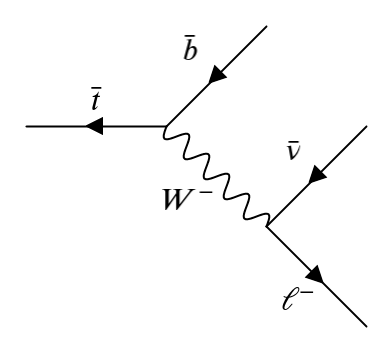
\includegraphics[width=\linewidth]{top3.png}
        \label{fig:top2}
    \end{minipage}
    \begin{minipage}{0.24\linewidth}
        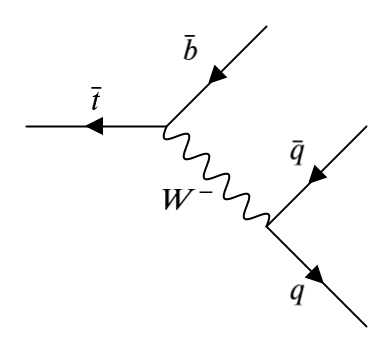
\includegraphics[width=\linewidth]{top4.png}
        \label{fig:anttop2}
    \end{minipage}
    \caption{Feynman diagrams of possible (anti-)top decays. From left to right, we see the top decay with leptonic final states, top decay with hadronic final states, anti-top decay with leptonic final states and anti-top decay with hadronic final states.}
    \label{fig:topdecay}
\end{figure}

%-------------------------------------------------------------------------%
\section{The Minimal Supersymmetric Standard Model}
The Minimal Supersymmetric Standard Model (MSSM) serves as an extension to the SM such that the particle content is duplicated once, thus keeping extra particles introduced to its minimum. Due to the symmetry groups of the SM being contained in the MSSM, any supersymmetric transformation would yield the same quantum numbers as that of the SM \cite{aitchison2007supersymmetry}. The fermions and bosons in the SM shown in Tables \ref{tab:SMFerm} and \ref{tab:SMBos}  have \textit{superpartners}; the supersymmetric counterparts to each particle in the SM as seen in Tables \ref{tab:SUSYspart} and \ref{tab:SUSYinos}. By convention the SM particles and their superpartners are distinguished by a tilde. \\

The MSSM relies on an extended theory to the SM known as the Two-Higgs-doublt model (2HDM), in which the SM Higgs consists of the up-type Higgs ($H_u$) and the down-type Higgs ($H_d$) that contain both neutral and charged components. The SM currently only has one Higgs doublet, giving rise to four degrees of freedom that produce the Higgs boson and the gauge bosons in the SM. In the 2HDM, the number of degrees of freedom doubles to eight, leading to 5 scalar components including the physical Higgs boson. In the MSSM, the superpartners of the Higgs, the Higgsinos, are the superpartners to the 2HDM, hence the two components in Table \ref{tab:SUSYinos}. \\

The superpartners to the SM particles are called \textit{squarks}, \textit{sleptons} and \textit{sneutrinos} whereas the superpartners to the bosons in the SM end with an ``-ino" e.g. \textit{gaugino}. The `symmetry' depicted in supersymmetry is the symmetry between fermions and bosons. This means that the fermions in the SM are bosons in the MSSM and vice versa \cite{martin1997supersymmetry}. Tables \ref{tab:SUSYspart} and \ref{tab:SUSYinos} illustrate that the number of new particles introduced is kept to a \textit{minimum} \cite{aitchison2007supersymmetry}. There is one problem, however. This symmetry we see in Tables \ref{tab:SMFerm}-\ref{tab:SUSYinos} would require that these MSSM particles have the same masses as their SM counterparts. We know this not to be true simply from such particles not being observed in collider experiments thus far. The symmetry must be broken at some high energy scale in an unknown way, allowing these particles to acquire much heavier masses to their SM counterparts that is unobservable with current collider experiments. \\

\begin{table}[htbp]
    \centering
    \begin{tabular}{||c|c|c|c||}
    \hline
    & Gen1 & Gen2 & Gen3 \\
    \hline
    & \\[-2.7ex]
    \multirow{2}{1.4cm}{squarks} & $\Tilde{u}$ & $\Tilde{c}$ & \small$\Tilde{t}$ \\
     & $\Tilde{d}$ & $\Tilde{s}$ & $\Tilde{b}$ \\
    \hline
    
    \multirow{2}{1.4cm}{sleptons} & $\Tilde{e}$ & $\Tilde{\mu}$ & $\Tilde{\tau}$ \\
     & $\Tilde{\nu_e}$ & $\Tilde{\nu_\mu}$ & $\Tilde{\nu_\tau}$ \\
    \hline
    \end{tabular}
    \caption{The superpartners to the SM quarks and leptons as squarks and sleptons. From the top row, left to right, we have the sup, charm, stop, sdown, sstrange and sbottom quarks, followed by the selectron, smuon and stau for the charged sleptons and their associated sneutrinos as neutral sleptons. As these are bosons, they are now integer spin, namely spin-0 scalar particles.}
    \label{tab:SUSYspart}
\end{table}

\begin{table}[htbp]
    \centering
    \begin{tabular}{||c|c||}
    \hline 
       Gauginos  & Higgsinos \\
       \hline
        & \\[-2.5ex]
      $\Tilde{g}$, $\Tilde{B}$, $\Tilde{W}^0$, $\Tilde{W}^\pm$ & $\Tilde{H}_u$,  $\Tilde{H}_d$ \\
     \hline
    \end{tabular}
    \caption{The superpartners to the SM force carriers as gauginos and Higgsinos. The gauginos consist of the gluino, Bino, and Winos (neutral and charged), and the Higgsinos is a superpartner to the 2HDM Higgs with three neutral components ($\Tilde{h}^0$, $\Tilde{H}^0$ and $\Tilde{A}^0$) and two charged components ($\Tilde{H}^\pm$).}
    \label{tab:SUSYinos}
\end{table}

Further expanding on the particles in Table \ref{tab:SUSYinos}, the MSSM introduces dark matter candidates known as \textit{neutralinos}  and \textit{charginos}. These particles are formed as a mixture of the neutral ($\Tilde{H}^0$, $\Tilde{h}^0$, $ \Tilde{A}^0 $, $\Tilde{B}$ and $\Tilde{W}^0$) and charged components ($\Tilde{W}^\pm$ and $\Tilde{H}^\pm$) of the MSSM fermions (excluding the gluino) as shown in Figure \ref{fig:SUSY}. The four neutralinos denoted $\Tilde{\chi}_i^0$ where $i=1,2,3,4$ has four candidates with a mass hierarchy of $ m_{\Tilde{\chi}_1^0} < m_{\Tilde{\chi}_2^0} < m_{\Tilde{\chi}_3^0} < m_{\Tilde{\chi}_4^0}$ \cite{martin1997supersymmetry}. The lightest of the four, $\Tilde{\chi}_1^0$, is thought to be the lightest supersymmetric particle (LSP) which is absolutely stable, supporting the theoretical properties of a proposed dark matter in cosmology. This assumption holds only when \textit{R-parity}, a new form of fundamental symmetry in the MSSM discussed below, is conserved \cite{martin1997supersymmetry}. As $\Tilde{\chi}_i^0$) is the only neutralino that cannot decay, other heavier neutralinos may decay via, but not limited to, two-body decays. In collider experiments, the `detection' of these neutralinos rely on the missing energy of reconstructed SUSY event, much like the SM neutrinos. \\

\begin{figure}[htbp]
    \centering
    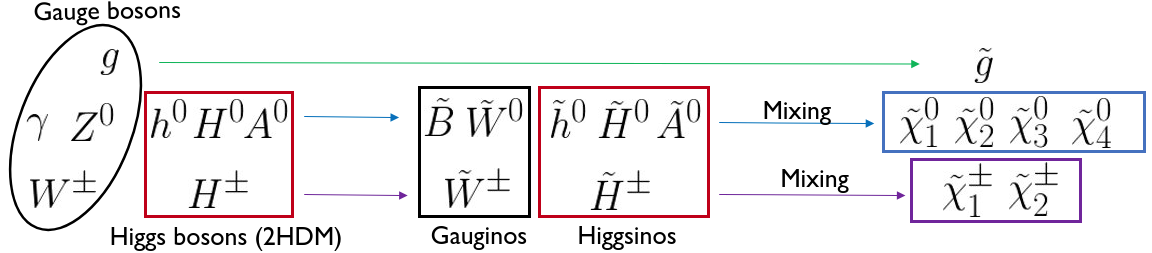
\includegraphics[width=\linewidth]{SUSY.png}
    \caption{Diagram depicting SM force carriers to their MSSM counterparts. The gluon is directly symmetric to the gluino, Higgs bosons and the W boson to the Higgsinos and the charged Winos, respectively. The photon and Z boson are technically part of the $B$ and the $W^3$, thus are symmetric to the Bino and neutral Wino, respectively. The neutral components of the gauginos and Higgsinos mix to give rise to the neutralinos, likewise for the charged components to the charginos.}
    \label{fig:SUSY}
\end{figure}

The new global symmetry \textit{R-parity} is required due to the the quantum numbers known as baryon ($B$) and lepton ($L$) numbers in the SM not considered as fundamental symmetries. This statement is supported by $B$- and $L$- violating processes that are strongly constrained by experiment. R-parity is a conserved quantum number given by Equation (\ref{eq:MPrec})
\begin{equation}
    P_R=(-1)^{3(B-L)+2s}
    \label{eq:MPrec}
\end{equation}
where $s$ is the spin of the particle. This symmetry conveniently separates SM particles and sparticles in a way that the SM particles have $P_R=+1$ (even R-parity), whereas the sparticles all have $P_R=-1$ (odd R-parity) \cite{martin1997supersymmetry}. In MSSM, the conservation of $R$-parity comes from SUSY events as a pair-produced event \cite{aitchison2007supersymmetry}. \\

%\footnote{The gauge invariance required in the SM ``accidentally" \cite{martin1997supersymmetry} guarantees the conservation of such quantum numbers in most interactions.}